\documentclass{config-wokSH}
\usepackage[spanish]{babel} % Idioma
%---------------------------- COMANDOS PORTADA ------------------/
%---------------------------------------------------------------/
%\newcommand*{\nombre}{Marco Silva Huerta}
\newcommand*{\fecha}{17 de Febrero de 2025}
\newcommand*{\semestre}{2025-2}
%\newcommand*{\id}{0000000}
\newcommand*{\nombreTarea}{Especificación de Requerimientos}
%\newcommand*{\subtitulo}{}
%---------------------------- COMANDOS PORTADA ----------------\
%---------------------------------------------------------------\


%-----------------------------------INICIO DE PACKETES-------------------/
%-----------------------------------------------------------------------/
\usepackage{amsmath}   % Matemáticas: Comandos extras(cajas ecuaciones) |
\usepackage{amsthm}
\usepackage{amssymb}   % Matemáticas: Símbolos matemáticos              |
\usepackage{datetime}  % Agregar fechas                                 |
\usepackage{graphicx}  % Insertar Imágenes                              |
\usepackage{multicol}  % Creación de tablas                             |
\usepackage{longtable} % Tablas más largas                              |
\usepackage{xcolor}    % Permite cambiar colores del texto              |
\usepackage{tcolorbox} % Cajas de color                                 |
\usepackage{setspace}  % Usar espacios                                  |
\usepackage{fancyhdr}  % Para agregar encabezado y pie de página        |
\usepackage{lastpage}  %                                                |
\usepackage{float}     % Flotantes                                      |
\usepackage{soul}      % "Efectos" en palabras                          |
\usepackage{hyperref}  % Para usar hipervínculos                        |
\usepackage{caption}   % Utilizar las referencias                       |
\usepackage{subcaption} % Poder usar subfiguras                         |
\usepackage{multirow}  % Nos permite modificar tablas                   |
\usepackage{array}     % Permite utilizar los valores para multicolumn  |
\usepackage{booktabs}  % Permite modificar tablas                       |
\usepackage{diagbox}   % Diagonales para las tablas                     |
\usepackage{colortbl}  % Color para tablas                              |
%\usepackage{listings}  % Escribir código                               |
\usepackage{mathtools} % SIMBOLO :=                                     |
\usepackage{enumitem}  % Modificar items de Listas                      |
\usepackage{tikz}      %                                                |
\usepackage{lipsum}    % for auto generating text                       |
\usepackage{afterpage} % for "\afterpage"s                              |
\usepackage{pagecolor} % With option pagecolor={somecolor or none}|     |
\usepackage{xpatch}    % Color de lineas C & F                          |
%\usepackage{glossaries} %                                              |
\usepackage{lastpage}  %                                                |
\usepackage{csquotes}  %                                                | 
\usepackage{array} % Paquete para definir el ancho de las columnas
%-----------------------------------------------------------------------\
%-----------------------------------FIN--- DE PACKETES-------------------\



%----------------------------------------------------------------------/
%-------------------Encabezado y Pie de Pagina-----------------------/ |
%--------------------------------------------------------------------\ |
%\fancyhf{}           %                                                |
%\pagestyle{fancy}

\fancypagestyle{firstpage}{  
    \fancyhead[L]{}
    \fancyhead[R]{}     
    \fancyfoot[L]{Equipo:\textsc{Bumper}}
    \fancyfoot[C]{}
    \fancyfoot[R]{\thepage\ de \pageref*{LastPage}}    
    \renewcommand{\headrulewidth}{0pt} 
    \xpretocmd\headrule{}{}{\PatchFailed}
}

\fancypagestyle{fancy}{  

    \fancyhead[L]{Requerimientos}
    \fancyhead[R]{}     

    \fancyfoot[L]{Equipo:\textsc{Bumper}}
    \fancyfoot[C]{}
    \fancyfoot[R]{\thepage\ de \pageref*{LastPage}}

    \renewcommand{\headrulewidth}{1pt} 
    \xpretocmd\headrule{}{}{\PatchFailed}
    \renewcommand{\footrulewidth}{1.5pt} 
    \xpretocmd\footrule{}{}{\PatchFailed}
}

%--------------------------------------------------------------------\ |
%-------------------Encabezado y Pie de Pagina-----------------------/ |
%------------------------------------------------------------FIN----/


\usepackage{tikz,times}
\usepackage{verbatim}
\usetikzlibrary{mindmap,trees,backgrounds}

%--------------------------------------------------------------------/
%------------------- LISTA DE COLORES ------------------------------/ 
\definecolor{ProcessBlue}{RGB}{0,176,240}
\definecolor{NavyBlue}{RGB}{0,110,184}
\definecolor{Cyan}{RGB}{0,174,239}
\definecolor{MidnightBlue}{RGB}{0,103,49}
\definecolor{ForestGreen}{RGB}{0,155,85}
\definecolor{Goldenrod}{RGB}{255,223,66}
\definecolor{YellowGreen}{RGB}{152,204,112}
\definecolor{Sepia}{RGB}{103,24,0}
\definecolor{Peach}{RGB}{247,150,90}
\definecolor{CarnationPink}{RGB}{242,130,180}
\definecolor{Fuchsia}{RGB}{140,54,140}
\definecolor{WildStrawberry}{RGB}{238,41,103}

\definecolor{Grass}{RGB}{41,238,53}
\definecolor{Meadow}{RGB}{6,243,67}
\definecolor{jellyfish}{RGB}{109,14,130}
\definecolor{rubber}{RGB}{229,27,232}
\definecolor{bullet}{RGB}{225,31,90}
\definecolor{midnight}{RGB}{31,90,225}
\definecolor{sun}{RGB}{241,152,7}
\definecolor{water}{RGB}{16,229,183}

%------------------- COLORES CÓDIGO -------------------- |

%------------------- COLORES JAVA ---------------------- |
\definecolor{backcolour}{RGB}{6,6,6} 
%\definecolor{backcolour}{RGB}{181,181,181} 
\definecolor{codeclassjava}{RGB}{246,113,59}
\definecolor{codegreen}{RGB}{17,225,48}
\definecolor{codenumizq}{RGB}{17,17,17}
\definecolor{codestringjava}{RGB}{51,240,234}
\definecolor{codesymboljava}{RGB}{255,5,0} 
\definecolor{yellowpoint}{RGB}{244,235,100} 
%------------------- COLORES JAVA ---------------------- |


%------------------- COLORES PYTHON -------------------- |
\definecolor{backcolourPY}{RGB}{6,6,6} 
%\definecolor{backcolour}{RGB}{181,181,181} 
\definecolor{codegreenPY}{RGB}{17,225,48}
\definecolor{codeclassPY}{RGB}{246,113,59}
\definecolor{codenumizq}{RGB}{17,17,17}
\definecolor{codestringPY}{RGB}{90,128,220}
\definecolor{codesymboljava}{RGB}{255,5,0} 
%------------------- COLORES PYTHON -------------------- |


%------------------- COLORES CÓDIGO -------------------- |

%------------------- LISTA DE COLORES -------------------------------\
%---------------------------------------------------------------------\


\usepackage[backend=biber]{biblatex}
\addbibresource{bibliografia.bib}

\nocite{*} % Añade todas las referencias de bib sin cita


% -------------------------------------------------------/
% ------------------------------------------------------/
\begin{document}

\pagestyle{fancy}

\thispagestyle{firstpage}
% -----------------|
% Portada Titulo   |
\maketitle %       |
% -----------------|
\tableofcontents

\section{Introducción}

Proyecto: \textbf{Bumper}

\begin{itemize}
    \item Aplicación web para el registro y visualización de incidentes urbanos.

    \item Bumper planea ser una herramienta colaborativa para mejorar comunicación ciudadana.

    \item Permitirá a ciudadanos, comerciantes y organizaciones vecinales participar activamente en seguimiento de reportes.
\end{itemize}

\subsection*{Requisitos del cliente}

\begin{itemize}
    \item \textbf{Registro de incidentes}
    \begin{itemize}
        \item Permitir a los usuarios marcar la ubicación del incidente en un mapa interactivo.
        \item Adjuntar una o más fotografías que respalden el incidente reportado.
        \item Registrar una breve descripción del problema.
    \end{itemize}
    \item \textbf{Actualización de estado del incidente}
    \begin{itemize}
        \item Permitir que cualquier usuario (no solo el creador del reporte) actualice el estado del incidente a "Resuelto", siempre que adjunte pruebas fotográficas que validen la solución.
    \end{itemize}
    \item \textbf{Visualización de incidentes}
    \begin{itemize}
        \item Mostrar todos los incidentes en un mapa interactivo, categorizados por tipo y estado (Reportado, En proceso, Resuelto).
    \end{itemize}
\end{itemize}
\section{Benchmark}

Este paso lo hemos completado para conocer las \textbf{soluciones actuales} en el mundo, conocer las fortalezas, debilidades, las formas de trabajo, conocer de sus interfaces y procesos. Con esta información tendremos un panorama de lo que ya existe y podremos hacer un camino de usuario para lograr una experiencia más amigable de nuestra aplicación. 

\begin{table}[h!]
\centering
\begin{tabular}{|>{\centering\arraybackslash}m{2.5cm}|>{\centering\arraybackslash}m{3cm}|>{\centering\arraybackslash}m{2.5cm}|>{\centering\arraybackslash}m{3cm}|>{\centering\arraybackslash}m{3cm}|} % Definir ancho de columna y centrar texto
\hline
\textbf{} & \textbf{FixMyStreet (Reino Unido)} & \textbf{SeeClickFix (EE.UU.)} & \textbf{Mejora tu Ciudad} & \textbf{Colab.re (Brasil)} \\ \hline
\textbf{Marcación en mapa} & Sí (OpenStreetMap) & Sí (Google Maps) & Sí (Google Maps) & Sí (Leaflet/OpenStreetMap) \\ \hline
\textbf{Adjuntar fotos} & Sí (1+ imágenes) & Sí (hasta 5 imágenes) & Sí (fotos y videos) & Sí (3+ imágenes) \\ \hline
\textbf{Descripción breve} & Texto libre & Campos predefinidos + texto & Texto libre & Texto + etiquetas \\ \hline
\textbf{Actualización de estado} & No (solo creador/autoridades) & Sí (usuarios verificados) & Sí (usuarios y autoridades) & Sí (usuarios registrados) \\ \hline
\textbf{Visualización de incidentes} & Mapa con filtros & Mapa interactivo con capas & Mapa con íconos & Mapa con filtros y heatmaps \\ \hline
\textbf{API del mapa} & OpenLayers + OpenStreetMap & Google Maps API + Esri & Google Maps API & Leaflet API + OpenStreetMap \\ \hline
\textbf{Tecnología} & Perl, PostgreSQL, OpenLayers & React, Node.js, AWS &  MySQL/Firebase  & JavaScript, Python, PostgreSQL \\ \hline
\textbf{Disponibilidad} & Reino Unido, Australia & EE.UU., Canadá &  España, México  & Brasil, Argentina, Uruguay \\ \hline
\end{tabular}
\caption{Comparativa de plataformas de gestión de incidentes urbanos}
\label{tab:comparativa}
\end{table}

\subsection*{Enlaces a las páginas}
\begin{minipage}[t]{0.48\textwidth}
\begin{itemize}
    \item \href{https://www.fixmystreet.com/}{FixMyStreet (Reino Unido)}
    \item \href{https://play.google.com/store/apps/details?id=com.seeclickfix.ma.android&hl=es_MX}{SeeClickFix (EE.UU.)}
\end{itemize}
\end{minipage}
\hfill
\begin{minipage}[t]{0.48\textwidth}
\begin{itemize}
    \item \href{https://mejoratuciudad.org/}{Mejora tu Ciudad (España)}
    \item \href{https://www.colab.com.br/sou-cidadao/}{Colab.re (Brasil)}
\end{itemize}
\end{minipage}


\begin{table}[H]
\centering
\begin{tabular}{|>{\centering\arraybackslash}m{2.7cm}|>{\centering\arraybackslash}m{3cm}|>{\centering\arraybackslash}m{3cm}|>{\centering\arraybackslash}m{3cm}|>{\centering\arraybackslash}m{3cm}|>{\centering\arraybackslash}m{3cm}|}
\hline
\textbf{} & \textbf{FixMyStreet (UK)} & \textbf{SeeClickFix (EEUU)} & \textbf{Mejora tu Ciudad (ES)} & \textbf{Colab.re (BR)} \\ \hline

\textbf{Fortalezas} & 
Integración autoridades \newline Open-source \newline PostgreSQL robusto & 
Interfaz intuitiva \newline Colaboración real-time \newline Escalabilidad AWS & 
Multimedia completo \newline Flexibilidad descripciones & 
Visualización avanzada \newline Stack moderno \newline Foco LATAM \\ \hline

\textbf{Debilidades} & 
Actualizaciones limitadas \newline Alcance reducido & 
APIs pagas \newline Límite imágenes & 
Tecnología oculta \newline Cobertura indefinida & 
Baja visibilidad global \newline Registro obligatorio \\ \hline

\textbf{Base de datos} & 
PostgreSQL & 
AWS RDS \newline(MySQL/PG) & 
MySQL/Firebase & 
PostgreSQL \\ \hline

\textbf{Propuesta de valor} & 
Comunicación simple \newline ciudadano-gobierno & 
Transparencia mediante \newline reportes verificados & 
Empoderamiento ciudadano \newline con evidencia visual & 
Soluciones basadas \newline en datos LATAM \\ \hline

\end{tabular}
\caption{Comparativa de puntos específicos}
\label{tab:comparativa-optimizada}
\end{table}

\section{Requerimientos}

\subsection*{Requerimientos Funcionales}

\begin{enumerate}
    \item \textbf{Autenticación de Usuarios (RF1)}
    \begin{itemize}
        \item El usuario puede registrarse e iniciar sesión con un correo electrónico y contraseña.
        \item Solo los usuarios autenticados pueden crear y modificar reportes.
    \end{itemize}

    \item \textbf{Gestión de Incidentes (RF2)}
    \begin{itemize}
        \item El usuario puede crear un reporte con ubicación, tipo de incidente, descripción y hasta 3 fotos.
        \item El usuario creador puede actualizar el estatus del reporte (``No resuelto'', ``En proceso'', ``Resuelto'').
        \item Los reportes incluyen un código único para seguimiento.
    \end{itemize}

    \item \textbf{Integración con Mapa Interactivo (RF3)}
    \begin{itemize}
        \item El usuario visualiza un mapa con marcadores de incidentes existentes.
        \item El usuario puede marcar una ubicación en el mapa al crear un reporte, con opción de escribir una dirección.
        \item El mapa permite zoom y arrastre para explorar áreas.
    \end{itemize}

    \item \textbf{Filtrado de Incidentes (RF4)}
    \begin{itemize}
        \item El usuario puede filtrar incidentes en el mapa por estatus (``Todos'', ``No resuelto'', etc.) y tipo de incidente (e.g., Bache, Basura).
    \end{itemize}

    \item \textbf{Visualización de Información (RF5)}
    \begin{itemize}
        \item El usuario ve una pantalla principal con el mapa y un botón para reportar.
        \item Al hacer clic en un marcador, se muestra una ventana con fotos, estatus y tipo de incidente.
        \item Una barra lateral ofrece el formulario para crear reportes y opciones de filtrado.
    \end{itemize}
\end{enumerate}

\subsection*{Requerimientos No Funcionales}

\begin{enumerate}
    \item \textbf{Seguridad (RNF1)}
    \begin{itemize}
        \item Las contraseñas y correos de los usuarios están protegidos con cifrado.
        \item Solo el creador puede modificar su reporte, garantizando control de acceso.
    \end{itemize}

    \item \textbf{Rendimiento (RNF2)}
    \begin{itemize}
        \item El mapa carga rápidamente y responde con baja latencia al interactuar.
        \item La aplicación soporta múltiples usuarios creando reportes al mismo tiempo.
    \end{itemize}

    \item \textbf{Disponibilidad (RNF3)}
    \begin{itemize}
        \item La solución funciona inicialmente en un entorno local o en un servidor básico.
    \end{itemize}

    \item \textbf{Usabilidad (RNF4)}
    \begin{itemize}
        \item La interfaz se adapta a diferentes dispositivos (móviles y escritorio).
        \item El diseño es claro, con navegación sencilla y acciones intuitivas.
    \end{itemize}

    \item \textbf{Escalabilidad (RNF5)}
    \begin{itemize}
        \item La aplicación permite añadir nuevas funcionalidades sin rediseños complejos.
        \item El almacenamiento de datos y fotos puede crecer según la demanda.
    \end{itemize}
\end{enumerate}
\section{Casos de Uso}

\subsection*{CU1: Hacer Login}
\textbf{Actores:} Usuario, Sistema\\
\textbf{Flujo Principal:}
\begin{enumerate}
    \item El usuario accede a la página de inicio de sesión. (RF1)
    \item Ingresa su correo electrónico y contraseña.
    \item El sistema verifica las credenciales.
    \item Si las credenciales son correctas, el usuario es redirigido al mapa principal. (RF5)
\end{enumerate}
\textbf{Flujo Alternativo:}
\begin{itemize}
    \item \textit{Credenciales incorrectas:}
    \begin{enumerate}
        \item El sistema muestra un mensaje de error indicando que las credenciales no son válidas.
        \item Ofrece un enlace para recuperar la contraseña por correo.
    \end{enumerate}
\end{itemize}


\subsection*{CU2: Reportar Incidente Urbano}
\textbf{Actores:} Ciudadano, Sistema\\
\textbf{Flujo Principal:}
\begin{enumerate}
    \item El usuario inicia sesión. (RF1)
    \item Hace clic en ``Reportar Incidente'' desde el mapa principal. (RF3)
    \item Marca la ubicación en el mapa o escribe una dirección. (RF3)
    \item Completa un formulario con tipo de incidente, descripción y hasta 3 fotos. (RF2)
    \item Confirma el reporte tras ver una vista previa.
    \item El sistema muestra el reporte en el mapa con un código único. (RF5)
\end{enumerate}
\textbf{Flujo Alternativo:}
\begin{itemize}
    \item \textit{Sin inicio de sesión:}
    \begin{enumerate}
        \item El sistema redirige al usuario a la página de inicio de sesión antes de continuar.
    \end{enumerate}
\end{itemize}

\subsection*{CU3: Modificar Estatus de Reporte}
\textbf{Actores:} Ciudadano (creador del reporte), Sistema\\
\textbf{Flujo Principal:}
\begin{enumerate}
    \item El usuario inicia sesión y selecciona uno de sus reportes en el mapa. (RF2)
    \item Abre la ventana del reporte y elige un nuevo estatus (``En proceso'' o ``Resuelto''). (RF2)
    \item Confirma el cambio.
    \item El sistema actualiza el estatus y muestra la versión modificada en el mapa. (RF5)
\end{enumerate}
\textbf{Flujo Alternativo:}
\begin{itemize}
    \item \textit{Usuario no creador:}
    \begin{enumerate}
        \item El sistema no muestra opciones de edición y limita la interacción a solo visualización.
    \end{enumerate}
\end{itemize}


\subsection*{CU4: Ver Detalles de un Incidente}
\textbf{Actores:} Usuario (registrado o invitado), Sistema\\
\textbf{Flujo Principal:}
\begin{enumerate}
    \item El usuario accede al mapa principal. (RF3)
    \item Hace clic en un marcador de incidente en el mapa.
    \item El sistema muestra una ventana emergente con los detalles del incidente, incluyendo:
    \begin{itemize}
        \item Tipo de incidente.
        \item Ubicación.
        \item Estado actual (Pendiente, En proceso, Resuelto).
        \item Fotos asociadas al incidente.
        \item Fecha y hora del reporte.
    \end{itemize}
\end{enumerate}
\textbf{Flujo Alternativo:}
\begin{itemize}
    \item \textit{Incidente sin fotos:}
    \begin{enumerate}
        \item El sistema muestra un mensaje indicando que no hay fotos disponibles para este incidente.
    \end{enumerate}
\end{itemize}

\subsection*{CU5: Editar Perfil de Usuario}
\textbf{Actores:} Usuario, Sistema\\
\textbf{Flujo Principal:}
\begin{enumerate}
    \item El usuario inicia sesión en el sistema. (RF1)
    \item Accede a la sección de "Perfil" desde el menú principal. (RF10)
    \item Visualiza su información actual, como nombre, apellido, correo electrónico y contraseña.
    \item Realiza cambios en los campos permitidos (por ejemplo, nombre o contraseña).
    \item Confirma los cambios haciendo clic en "Guardar". (RF11)
    \item El sistema valida los datos ingresados y actualiza la información en la base de datos.
    \item El sistema muestra un mensaje de confirmación indicando que los cambios se han guardado correctamente.
\end{enumerate}
\textbf{Flujo Alternativo:}
\begin{itemize}
    \item \textit{Datos inválidos:}
    \begin{enumerate}
        \item El sistema muestra un mensaje de error indicando qué campos necesitan corrección.
        \item El usuario corrige los datos y vuelve a intentar guardar los cambios.
    \end{enumerate}
\end{itemize}
\section{Tecnología Usada}


\subsection*{Backend}
\begin{itemize}
    \item \textbf{Lenguaje de Programación: Kotlin}
    \begin{itemize}
        \item \textit{Razón de uso:} Kotlin es un lenguaje moderno, conciso y seguro que mejora la productividad del desarrollo al reducir el código repetitivo y minimizar errores comunes (como null pointer exceptions). Su interoperabilidad con Java permite aprovechar bibliotecas existentes, mientras que su sintaxis clara facilita el mantenimiento del código.
        \item \textit{Ventaja para Bumper:} Ideal para implementar una API RESTful robusta (RF2, RF3) que gestione autenticación (RF1) y modificaciones de reportes (CU3), asegurando un backend eficiente y fácil de escalar (RNF5).
    \end{itemize}
    \item \textbf{Framework: Spring Boot}
    \begin{itemize}
        \item \textit{Razón de uso:} Spring Boot simplifica la creación de aplicaciones backend con configuraciones automáticas, integración nativa con bases de datos y soporte para seguridad. Su arquitectura basada en microservicios permite manejar solicitudes simultáneas con baja latencia (RNF2).
        \item \textit{Ventaja para Bumper:} Facilita la gestión de reportes (RF2) y la autenticación de usuarios (CU1), ofreciendo un entorno estable y modular que puede crecer con nuevas funcionalidades, como notificaciones o integración con autoridades (RNF5).
    \end{itemize}
\end{itemize}

\subsection*{Frontend}
\begin{itemize}
    \item \textbf{React}
    \begin{itemize}
        \item \textit{Razón de uso:} React es una biblioteca de JavaScript que permite construir interfaces dinámicas y responsivas (RNF4) mediante componentes reutilizables. Su enfoque en el estado y la renderización eficiente soporta interacciones en tiempo real, como filtros en el mapa (RF4) y vistas previas de reportes (CU2).
        \item \textit{Ventaja para Bumper:} Perfecto para integrar un mapa interactivo (RF3) y una barra lateral dinámica (CU4), asegurando una experiencia de usuario intuitiva y adaptable a dispositivos móviles (RNF4). Además, su ecosistema (e.g., react-leaflet) simplifica la integración con mapas.
    \end{itemize}
\end{itemize}

\subsection*{Base de Datos}
\begin{itemize}
    \item \textbf{PostgreSQL en Supabase}
    \begin{itemize}
        \item \textit{Razón de uso:} PostgreSQL es un sistema de base de datos relacional robusto y de código abierto, ideal para almacenar datos estructurados como reportes con ubicaciones, estatus y fotos (RF2). Supabase añade una capa de facilidad con almacenamiento de archivos (fotos) y autenticación integrada, reduciendo la complejidad inicial.
        \item \textit{Ventaja para Bumper:} Garantiza la persistencia de los reportes (CU2, CU3) y permite consultas rápidas para filtros (RF4), con escalabilidad para soportar más usuarios y datos (RNF5). El uso de Supabase ofrece un nivel gratuito inicial, optimizando costos para el prototipo y el que este activo siempre nos da cierta ventaja.
    \end{itemize}
\end{itemize}

\subsection*{API para Mapas}
\begin{itemize}
    \item \textbf{Leaflet con OpenStreetMap (Opción Principal)}
    \begin{itemize}
        \item \textit{Razón de uso:} Leaflet es una biblioteca ligera y de código abierto para mapas interactivos, combinada con OpenStreetMap, una fuente de datos gratuita y global. Esto permite visualizar y marcar incidentes (RF3) sin costos asociados, a diferencia de APIs comerciales.
        \item \textit{Ventaja para Bumper:} Su integración con React (via react-leaflet) asegura un mapa fluido y personalizable (CU4), con filtros dinámicos (RF4) y baja latencia (RNF2). Es ideal para un MVP escalable y económico (RNF5), con soporte para marcadores y popups (CU2, CU3).
    \end{itemize}
    \item \textbf{Google Maps API (Alternativa)}
    \begin{itemize}
        \item \textit{Razón de uso:} Ofrece funcionalidades avanzadas como autocompletado de direcciones y alta calidad visual, útil si se prioriza una experiencia premium en el futuro.
        \item \textit{Ventaja para Bumper:} Podría mejorar la precisión de ubicaciones (CU2), pero su costo (crédito limitado de \$200/mes) lo hace menos viable para la fase inicial frente a Leaflet.
    \end{itemize}
\end{itemize}
\newpage
\section{Diagramas}

\subsubsection*{Acceso y Registro de Usuario}
\begin{center}
    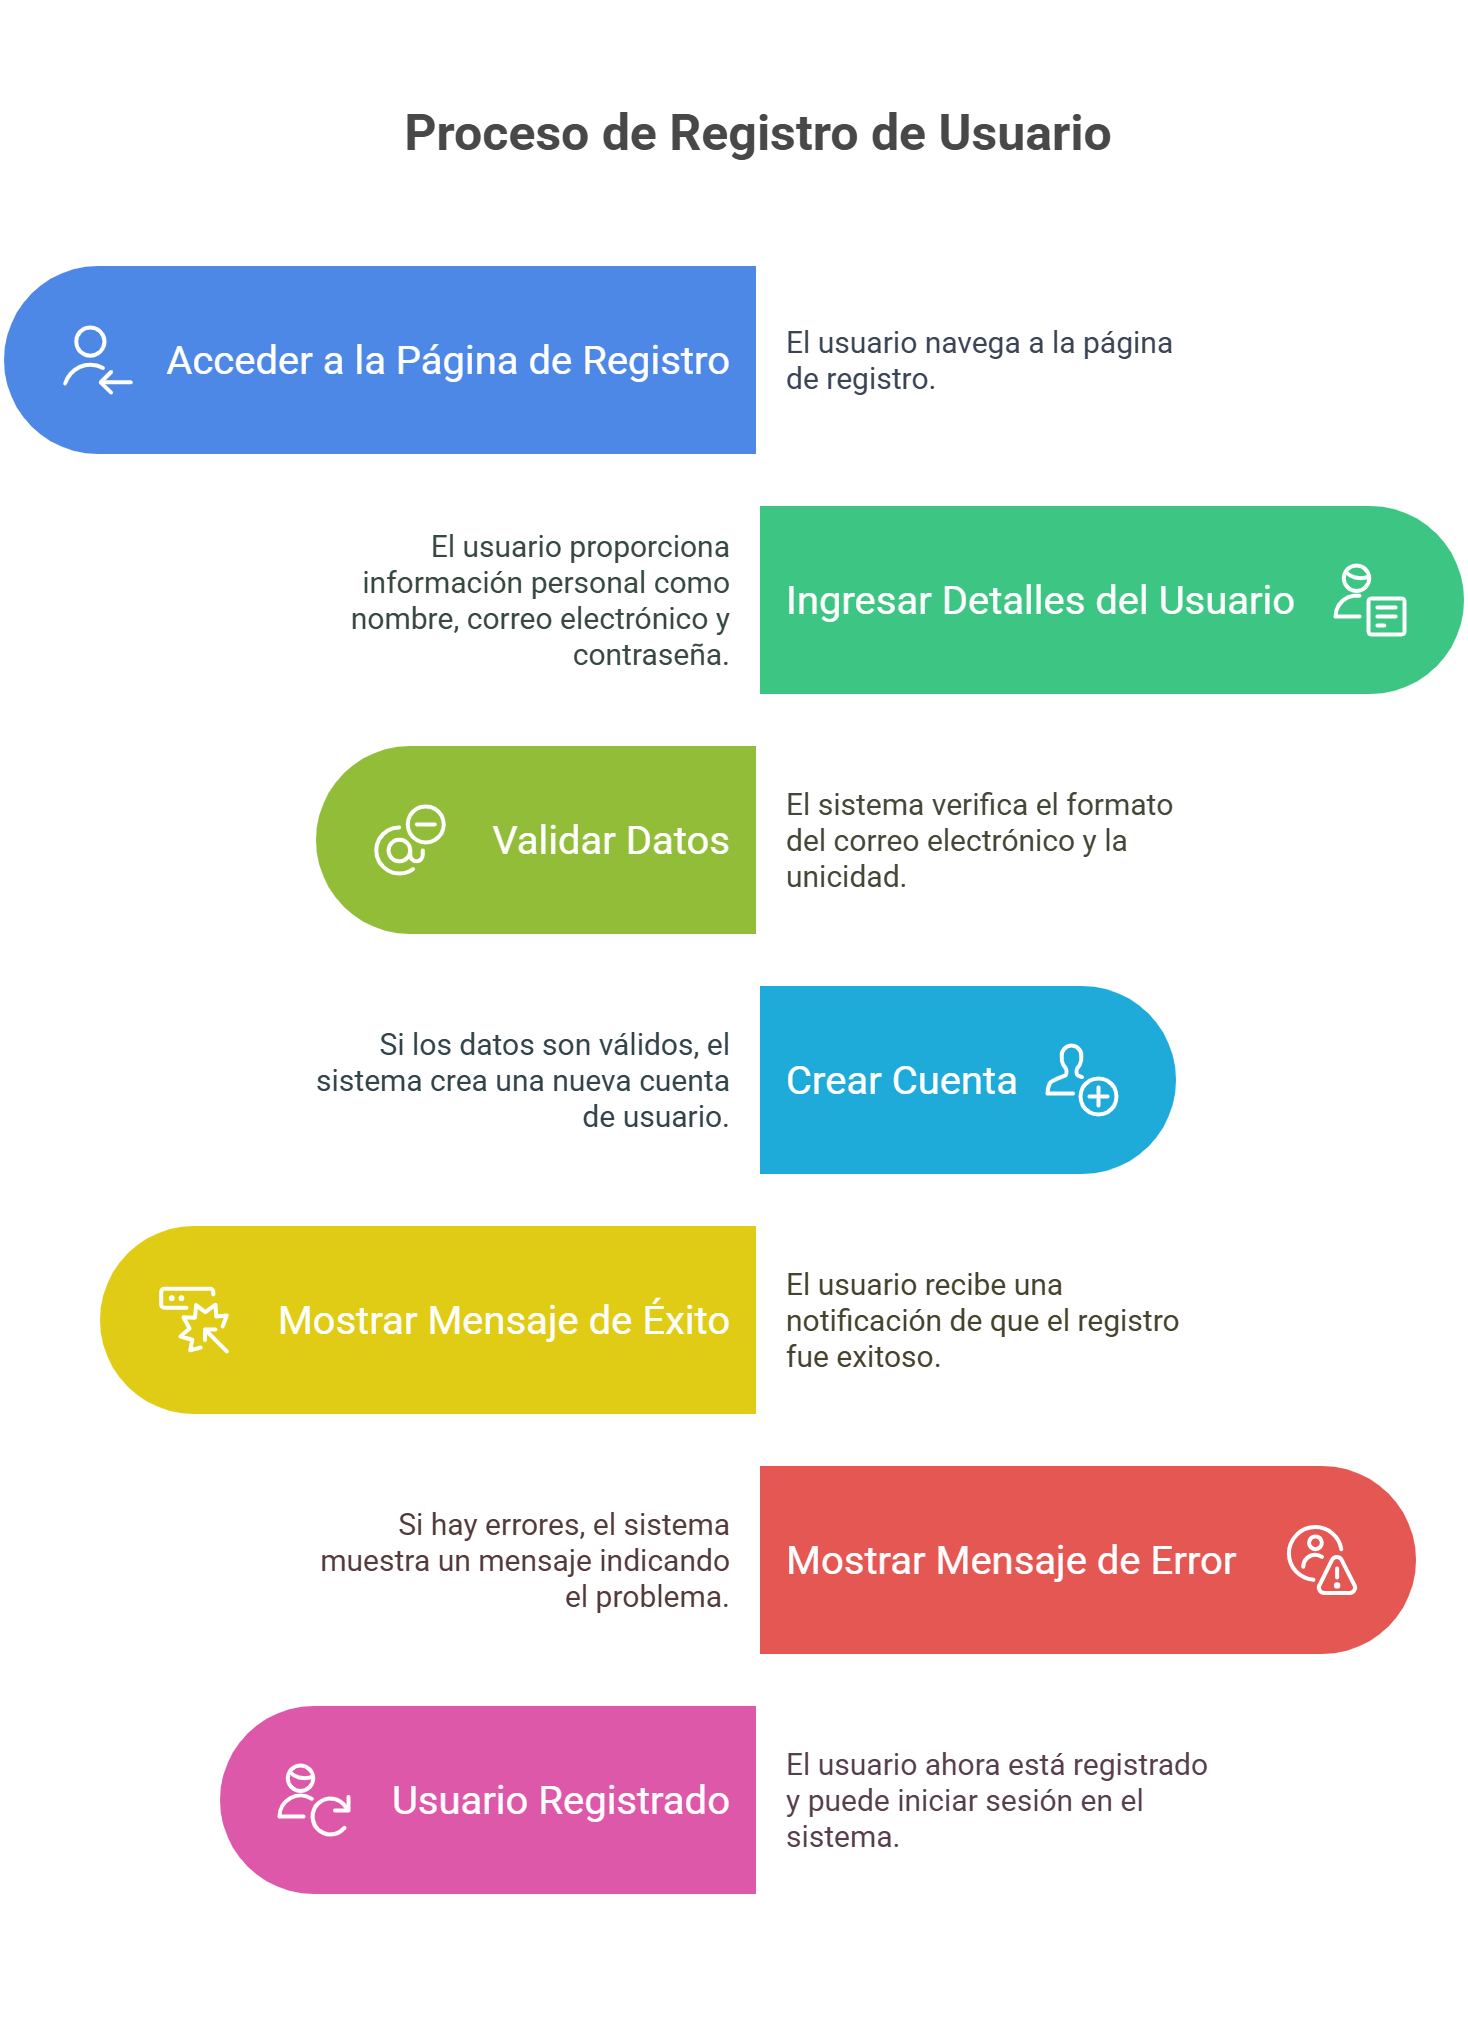
\includegraphics[scale = .3]{IMA/flujosUsuario/Acceso y Registro de Usuario.png}
\end{center}

\newpage
\subsubsection*{Inicio de Sesión}
\begin{center}
    \includegraphics[scale = .3]{IMA/flujosUsuario/Inicio de Sesión.png}
\end{center}

\newpage
\subsubsection*{Creación de Reporte de Incidente}
\begin{center}
    \includegraphics[scale = .3]{IMA/flujosUsuario/Creación de Reporte de Incidente.png}
\end{center}

\newpage
\subsubsection*{Consulta y Gestión de Mis Reportes}
\begin{center}
    \includegraphics[scale = .25]{IMA/flujosUsuario/Consulta y Gestión de Mis Reportes.png}
\end{center}

\newpage
\subsubsection*{Visualización de Incidentes en el Mapa}
\begin{center}
    \includegraphics[scale = .35]{IMA/flujosUsuario/Visualización de Incidentes en el Mapa.png}
\end{center}

\newpage
\subsubsection*{Cierre de Sesión}
\begin{center}
    \includegraphics[scale = .31]{IMA/flujosUsuario/Cierre de Sesión.png}
\end{center}

\newpage
\subsubsection*{Cambio de Contraseña}
\begin{center}
    \includegraphics[scale = .3]{IMA/flujosUsuario/Cambio de Contraseña.png}
\end{center}

\newpage
\subsubsection*{Descarga de Reporte}
\begin{center}
    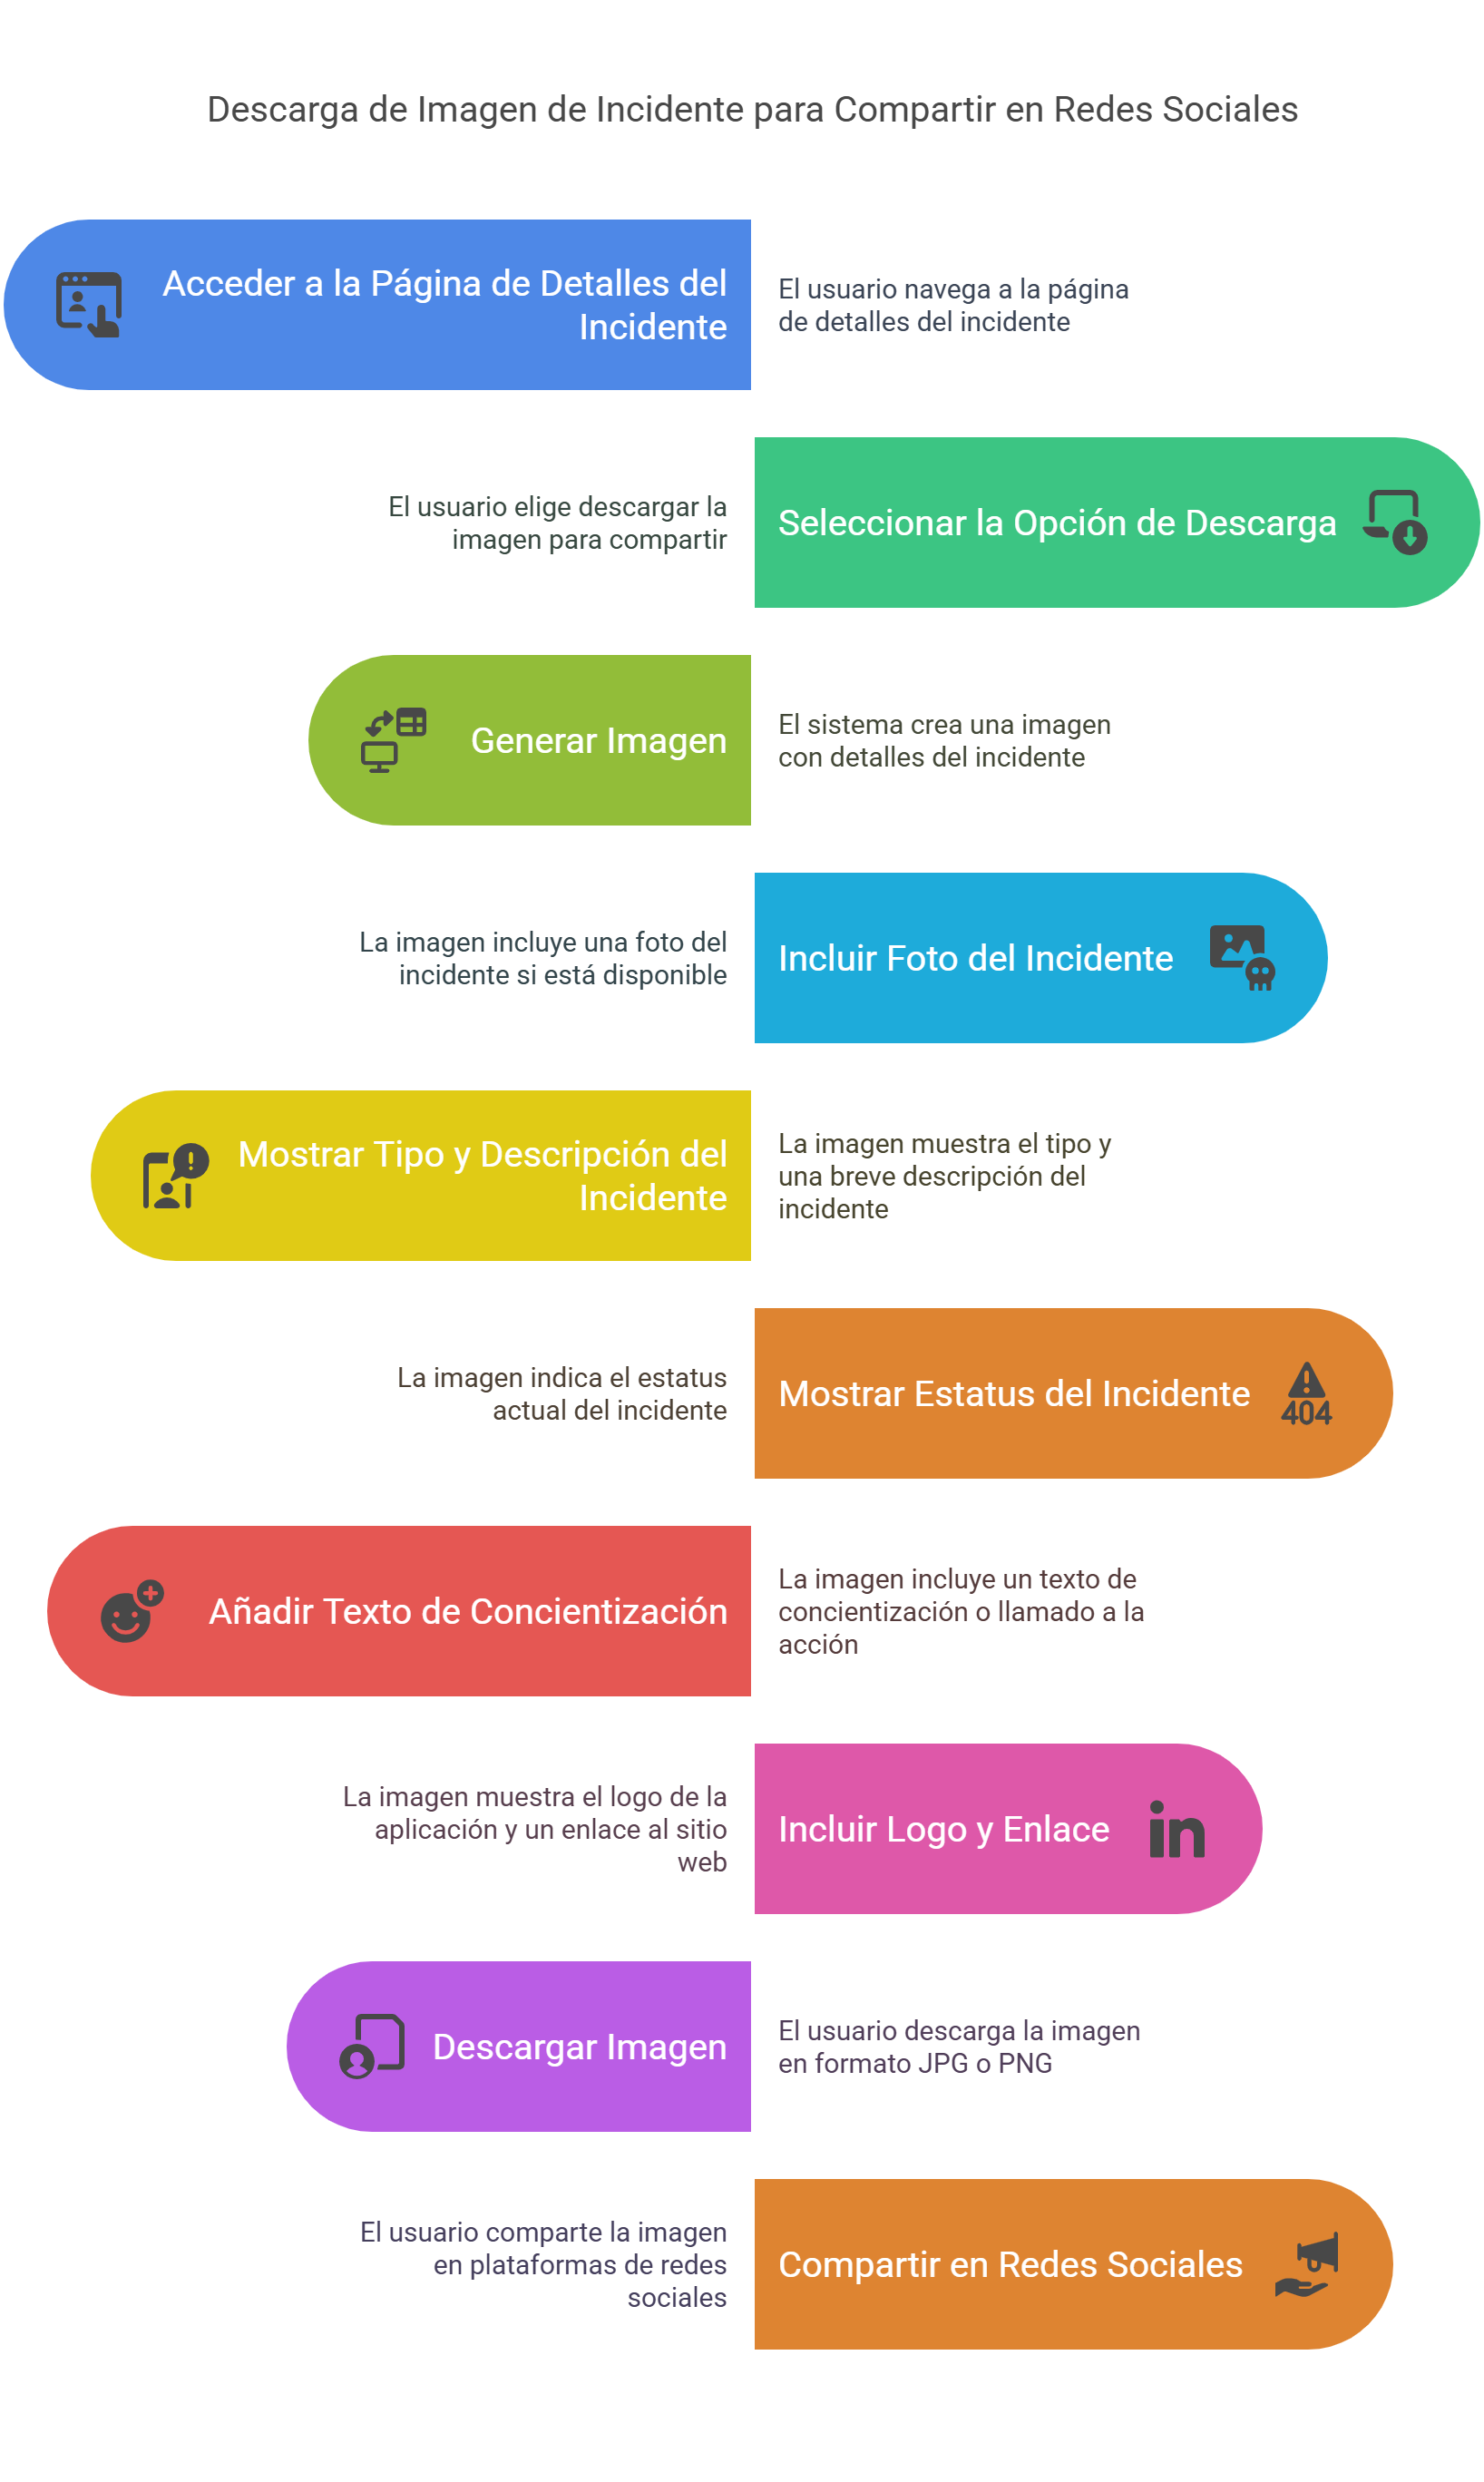
\includegraphics[scale = .25]{IMA/flujosUsuario/Descarga de Reporte.png}
\end{center}
\section{Documentación API}

\textbf{1. Crear un nuevo usuario}

\textit{Endpoint:} \texttt{POST /v1/users/create}

\textit{Descripción:} Crea un nuevo usuario en la base de datos.

\textit{Solicitud:}
\begin{itemize}
    \item \textbf{URL:} \texttt{http://localhost:8080/v1/users/create}
    \item \textbf{Método:} \texttt{POST}
    \item \textbf{Headers:} \texttt{Content-Type: application/json}
    \item \textbf{Body:}
\end{itemize}

\begin{lstlisting}
{
    "nombre": "Juan",
    "apellido": "Perez",
    "correo": "juan@example.com",
    "password": "1234",
    "token": "inactivo",
    "numeroIncidentes": 0
}
\end{lstlisting}

\textit{Respuesta esperada (éxito, HTTP 201):}
\begin{lstlisting}
{
    "id": 1,
    "nombre": "Juan",
    "apellido": "Perez",
    "correo": "juan@example.com",
    "password": "1234",
    "token": "inactivo",
    "numeroIncidentes": 0,
    "incidentes": []
}
\end{lstlisting}

\textit{Notas:}
\begin{itemize}
    \item El \texttt{id} será generado automáticamente por la base de datos
    \item \texttt{token} y \texttt{numeroIncidentes} tienen valores por defecto
\end{itemize}

\textbf{2. Iniciar sesión (Login)}

\textit{Endpoint:} \texttt{POST /v1/users/login}

\textit{Descripción:} Inicia sesión y cambia el token a \texttt{"activo"}.

\textit{Solicitud:}
\begin{itemize}
    \item \textbf{URL:} \texttt{http://localhost:8080/v1/users/login}
    \item \textbf{Método:} \texttt{POST}
    \item \textbf{Headers:} \texttt{Content-Type: application/json}
    \item \textbf{Body:}
\end{itemize}

\begin{lstlisting}
{
    "correo": "juan@example.com",
    "password": "1234"
}
\end{lstlisting}

\textit{Respuesta esperada (éxito, HTTP 200):}
\begin{lstlisting}
{
    "id": 1,
    "nombre": "Juan",
    "apellido": "Perez",
    "correo": "juan@example.com",
    "password": "1234",
    "token": "activo",
    "numeroIncidentes": 0,
    "incidentes": []
}
\end{lstlisting}

\textit{Notas:}
\begin{itemize}
    \item Credenciales incorrectas devuelven HTTP 401
\end{itemize}

\textbf{3. Crear un nuevo incidente}

\textit{Endpoint:} \texttt{POST /v1/incidentes}

\textit{Descripción:} Crea incidente asociado al usuario.

\textit{Solicitud:}
\begin{itemize}
    \item \textbf{URL:} \texttt{http://localhost:8080/v1/incidentes}
    \item \textbf{Método:} \texttt{POST}
    \item \textbf{Headers:} \texttt{Content-Type: application/json}
    \item \textbf{Body:}
\end{itemize}

\begin{lstlisting}
{
    "usuarioId": 1,
    "tipoIncidente": "BACHES",
    "ubicacion": "Av. Principal 123",
    "tipoVialidad": "AVENIDA"
}
\end{lstlisting}

\textit{Respuesta esperada (éxito, HTTP 201):}
\begin{lstlisting}
{
    "id": 1,
    "usuario": {
        "id": 1,
        "nombre": "Juan",
        "apellido": "Perez",
        "correo": "juan@example.com",
        "password": "1234",
        "token": "activo",
        "numeroIncidentes": 1,
        "incidentes": []
    },
    "tipoIncidente": "BACHES",
    "ubicacion": "Av. Principal 123",
    "horaIncidente": "2025-03-23T10:00:00",
    "tipoVialidad": "AVENIDA"
}
\end{lstlisting}

\textbf{4. Recuperar todos los incidentes}

\textit{Endpoint:} \texttt{GET /v1/incidentes}

\textit{Descripción:} Lista todos los incidentes en la base de datos.

\textit{Solicitud:}
\begin{itemize}
    \item \textbf{URL:} \texttt{http://localhost:8080/v1/incidentes}
    \item \textbf{Método:} \texttt{GET}
    \item \textbf{Headers:} (ninguno requerido)
    \item \textbf{Body:} (ninguno)
\end{itemize}

\textit{Respuesta esperada (éxito, HTTP 200):}
\begin{lstlisting}
[
    {
        "id": 1,
        "usuario": {
            "id": 1,
            "nombre": "Juan",
            "apellido": "Perez",
            "correo": "juan@example.com",
            "password": "1234",
            "token": "activo",
            "numeroIncidentes": 1,
            "incidentes": []
        },
        "tipoIncidente": "BACHES",
        "ubicacion": "Av. Principal 123",
        "horaIncidente": "2025-03-23T10:00:00",
        "tipoVialidad": "AVENIDA"
    }
]
\end{lstlisting}

\textit{Notas:}
\begin{itemize}
    \item Muestra todos los incidentes creados en el sistema
\end{itemize}

\textbf{5. Recuperar incidentes por usuario}

\textit{Endpoint:} \texttt{GET /v1/incidentes/usuario/\{usuarioId\}}

\textit{Descripción:} Lista incidentes asociados a un usuario específico.

\textit{Solicitud:}
\begin{itemize}
    \item \textbf{URL:} \texttt{http://localhost:8080/v1/incidentes/usuario/1}
    \item \textbf{Método:} \texttt{GET}
    \item \textbf{Headers:} (ninguno requerido)
    \item \textbf{Body:} (ninguno)
\end{itemize}

\textit{Respuesta esperada (éxito, HTTP 200):}
\begin{lstlisting}
[
    {
        "id": 1,
        "usuario": {
            "id": 1,
            "nombre": "Juan",
            "apellido": "Perez",
            "correo": "juan@example.com",
            "password": "1234",
            "token": "activo",
            "numeroIncidentes": 1,
            "incidentes": []
        },
        "tipoIncidente": "BACHES",
        "ubicacion": "Av. Principal 123",
        "horaIncidente": "2025-03-23T10:00:00",
        "tipoVialidad": "AVENIDA"
    }
]
\end{lstlisting}

\textit{Notas:}
\begin{itemize}
    \item El parámetro \texttt{\{usuarioId\}} debe coincidir con un ID existente
    \item Devuelve lista vacía si no hay incidentes asociados
\end{itemize}

\textbf{6. Obtener información del usuario (verificación)}

\textit{Endpoint:} \texttt{GET /v1/users/me}

\textit{Descripción:} Obtiene detalles del usuario con contador actualizado.

\textit{Solicitud:}
\begin{itemize}
    \item \textbf{URL:} \texttt{http://localhost:8080/v1/users/me}
    \item \textbf{Método:} \texttt{GET}
    \item \textbf{Headers:} \texttt{correo: juan@example.com}
    \item \textbf{Body:} (ninguno)
\end{itemize}

\textit{Respuesta esperada (éxito, HTTP 200):}
\begin{lstlisting}
{
    "id": 1,
    "nombre": "Juan",
    "apellido": "Perez",
    "correo": "juan@example.com",
    "password": "1234",
    "token": "activo",
    "numeroIncidentes": 1,
    "incidentes": []
}
\end{lstlisting}

\textit{Notas:}
\begin{itemize}
    \item Requiere header \texttt{correo} válido
    \item Verifica estado actual de \texttt{numeroIncidentes}
    \item Muestra información sensible como \texttt{password} (solo para fines demostrativos)
\end{itemize}

\textbf{7. Cerrar sesión (Logout)}

\textit{Endpoint:} \texttt{POST /v1/users/logout}

\textit{Descripción:} Cierra sesión cambiando token a \texttt{"inactivo"}.

\textit{Solicitud:}
\begin{itemize}
    \item \textbf{URL:} \texttt{http://localhost:8080/v1/users/logout}
    \item \textbf{Método:} \texttt{POST}
    \item \textbf{Headers:} \texttt{correo: juan@example.com}
    \item \textbf{Body:} (ninguno)
\end{itemize}

\textit{Respuesta esperada (éxito, HTTP 200):}
\begin{lstlisting}
"Sesion cerrada correctamente"
\end{lstlisting}

\textit{Notas:}
\begin{itemize}
    \item Cambia estado del token a inactivo
    \item Verificación posterior con \texttt{GET /v1/users/me} muestra nuevo estado
    \item Requiere mismo header \texttt{correo} usado en login
\end{itemize}
\section{Diagrama de Base de datos}

\begin{center}
    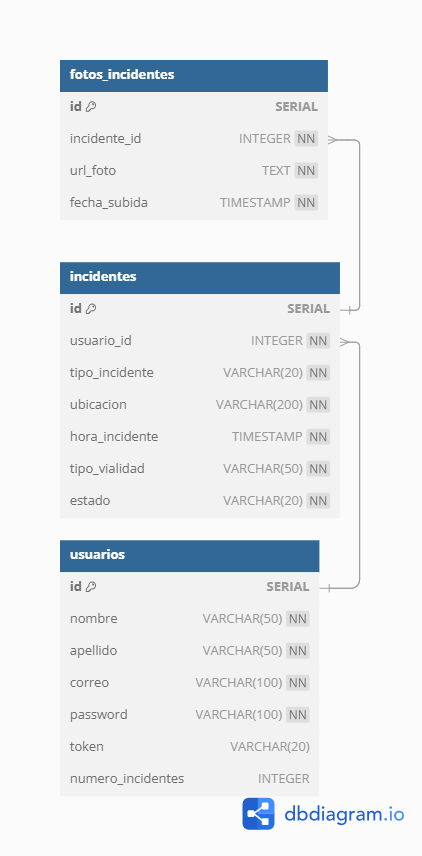
\includegraphics[scale = .7]{Ite02/SQL2.0.png}
\end{center}

% --------------------|
% Referencias         |
%\newpage %           |
%\printbibliography % |
% --------------------|

\end{document}
% -----------------------------------------------------\
% ------------------------------------------------------\